\documentclass[12pt,a4paper]{article}
\usepackage[margin=0.9in]{geometry}
\usepackage{booktabs}    % professional table lines
\usepackage{graphicx}    % for \includegraphics
\usepackage{float}       % for [H] table/figure placement
\usepackage{amsmath}     % for equations
\usepackage{tabularx}
\usepackage{caption}
\usepackage{siunitx}
\usepackage{threeparttable}

% --- Document body ---
\begin{document}
\title{CEDA Stata Test Answers}
\author{Anushka Gutte}
\maketitle


\section{Introduction}

This assignment uses Periodic Labour Force Survey (PLFS) 2017 data to examine consumption patterns, employment outcomes and wage disparities in India. All estimates use appropriate sampling weights, as laid out in the instruction manual.

\subsection{Consumption across States}

Table 1 presents the weighted average household consumption expenditure across states. The top states in terms of consumption are Chandigarh, Andaman \& Nicobar Islands, Delhi, Lakshadweep and Goa.

\begin{table}[H]
\centering
\caption{Average household consumption across states}
\begin{tabular}{clc}
\toprule
Rank & State & Average Household Consumption (Rs.) \\
\midrule
1&Chandigarh&17,014.61\\
2&Andaman \& Nicobar Islands&14,979.91\\
3&Delhi&14,517.24\\
4&Lakshadweep&14,418.77\\
5&Goa&13,507.59\\
6&Punjab&12,261.70\\
7&Pondicherry&12,056.21\\
8&Mizoram&10,910.77\\
9&Kerala&10,905.09\\
10&Haryana&10,849.47\\
\bottomrule
\end{tabular}
\end{table}
\label{tab:state_consumption}

\subsection{Deciles of household consumption expenditure}

 Table 2 reports the decile cut-offs for household consumption expenditure. The bottom decile ranges from approximately Rs. 250 to Rs. 3,000, while the top decile begins around Rs. 15,000 and extends significantly higher. The large gap between upper deciles reflects substantial inequality in consumption expenditure.

\vspace{1em}
\begin{table}[H]
\centering
\caption{Household consumption expenditure (Rs) in Deciles}
\begin{tabular}{clc}
\toprule
Decile & Min HH Consumption & Max HH Consumption  \\
\midrule
1&250.00&3,000.00\\
2&3,002.00&4,000.00\\
3&4,015.00&5,000.00\\
4&5,008.00&5,500.00\\
5&5,501.00&6,000.00\\
6&6,010.00&7,500.00\\
7&7,508.00&9,000.00\\
8&9,015.00&10,500.00\\
9&10,515.00&15,000.00\\
10&15,012.00&150,000.00\\
\bottomrule
\end{tabular}
\end{table}


\subsection{Gender differences in employment}

Table 3 presents the survey-weighted mean employment rates by sex for individuals aged 15–59. About 74.4\% of males are employed, compared to 21.3\% of females, highlighting a substantial gender employment gap. Transgender individuals have an employment rate of 31.3\%.

\begin{table}[htbp]
\centering
\caption{Weighted mean employment by sex}
\begin{tabular}{lc}
\toprule
Sex & Mean Employment \\
\midrule
Male&.744\\
Female&.213\\
Transgender&.313\\
\bottomrule
\end{tabular}
\end{table}


To formally assess the magnitude of this gap, the following linear regression model is estimated:

\begin{equation} Employed_i = \alpha + \beta Female_i + \epsilon_i \end{equation}
\vspace{-5pt}

\begin{table}[htbp]\centering
\def\sym#1{\ifmmode^{#1}\else\(^{#1}\)\fi}
\caption{Gender employment gap}
\begin{tabular}{l*{1}{c}}
\hline
                    &\multicolumn{1}{c}{(1)}\\
                    &\multicolumn{1}{c}{Employed}\\
                    &        b/se         \\
\hline
Female (1 = yes)    &      -0.530\sym{***}\\
                    &     (0.003)         \\
Constant            &       0.743\sym{***}\\
                    &     (0.002)         \\
\hline
N                   &     289,338         \\
\hline
\end{tabular}
\end{table}


Results from Table 4 imply that females are approximately 53 percentage points less likely to be employed compared to males. The difference is statistically significant at the 5\% level.

\subsection{Female employment across consumption deciles}

Figure 1 plots female employment rates by principal status across consumption deciles. The graph shows clear patterns. Casual wage labour dominates in the poorest deciles, with rates around 9.5\% in decile 1 and 7\% in decile 2, declining to near zero by decile 10. Regular salaried employment rises sharply with household wealth, from near zero in the poorest decile to about 8\% in the richest, reflecting that formal wage jobs are concentrated among wealthier women. Self-employment and unpaid family work remain relatively stable across deciles. This compositional shift highlights the need for policies that expand quality employment opportunities for women in the lower and middle consumption segments.

\begin{figure}[H]
    \centering
    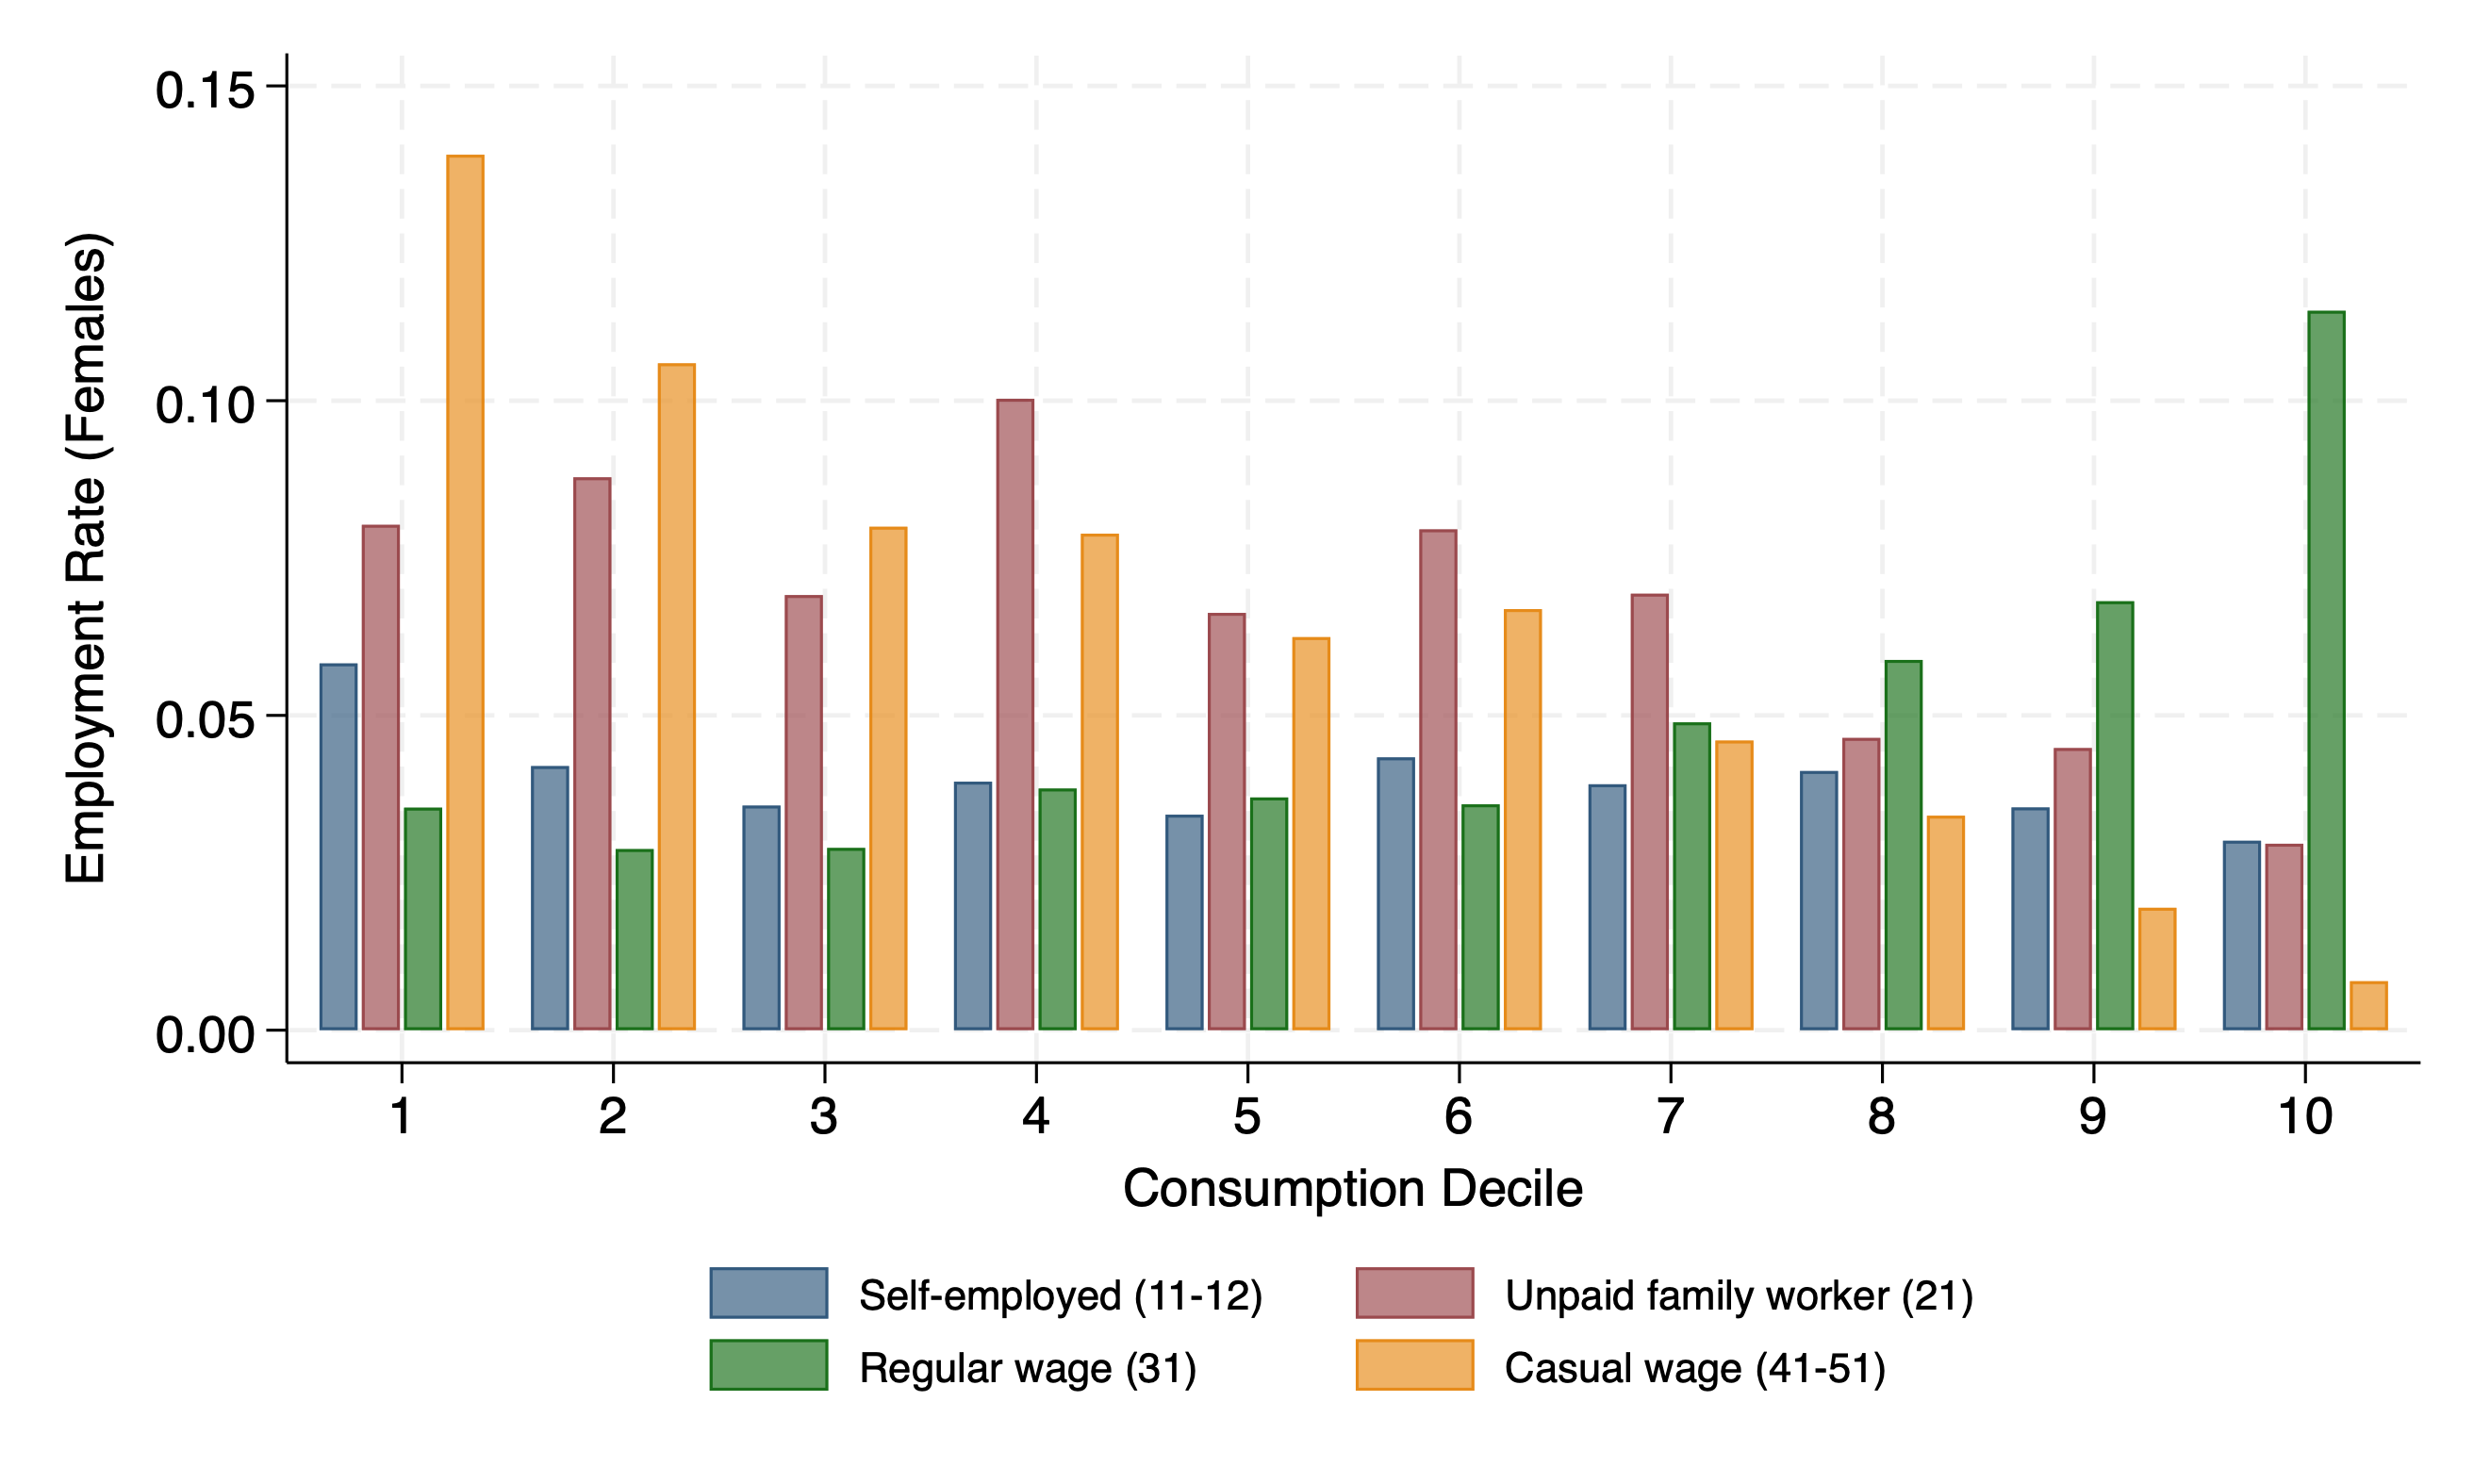
\includegraphics[scale=0.3]{female_emp_status_decile.png}
\caption{Female Employment by Principal Status and HH Consumption Decile}
\end{figure}

\subsection{Daily wage rates by employment type} 

Table 5 summarises the key statistics of daily wage rates for employed individuals by type of employment.

\begin{table}[htbp]\centering
\def\sym#1{\ifmmode^{#1}\else\(^{#1}\)\fi}
\caption{Daily wage rates by employment type}
\begin{tabular}{l*{1}{ccccc}}
\hline
                    &\multicolumn{5}{c}{}                                            \\
                    &        Mean&          SD&         Min&         Max&           N\\
\hline
Regular Salaried Wage&      545.65&      511.21&        0.00&    23333.33&       41867\\
Casual Worker Wage  &      266.04&      123.70&        0.00&     2333.33&       24416\\
Self-employed Wage  &        3.38&       26.94&        0.00&     1000.00&       63475\\
\hline
\end{tabular}
\end{table}



Regular salaried workers earn the highest wages on average, followed by casual workers. Methodologically, daily wages for salaried workers are computed by dividing monthly earnings by 30. For casual and self-employed workers, weekly earnings reported in the survey are used. This is likely why the mean for self-employed individuals is so low, as no alternative measure was available.

\subsection{Daily wage rate by caste status}

Figure 2 shows average daily wages by caste group.
General caste individuals earn higher wages on average, while SC/ST and OBC groups earn lower wages. 

\begin{figure}[H]
    \centering
    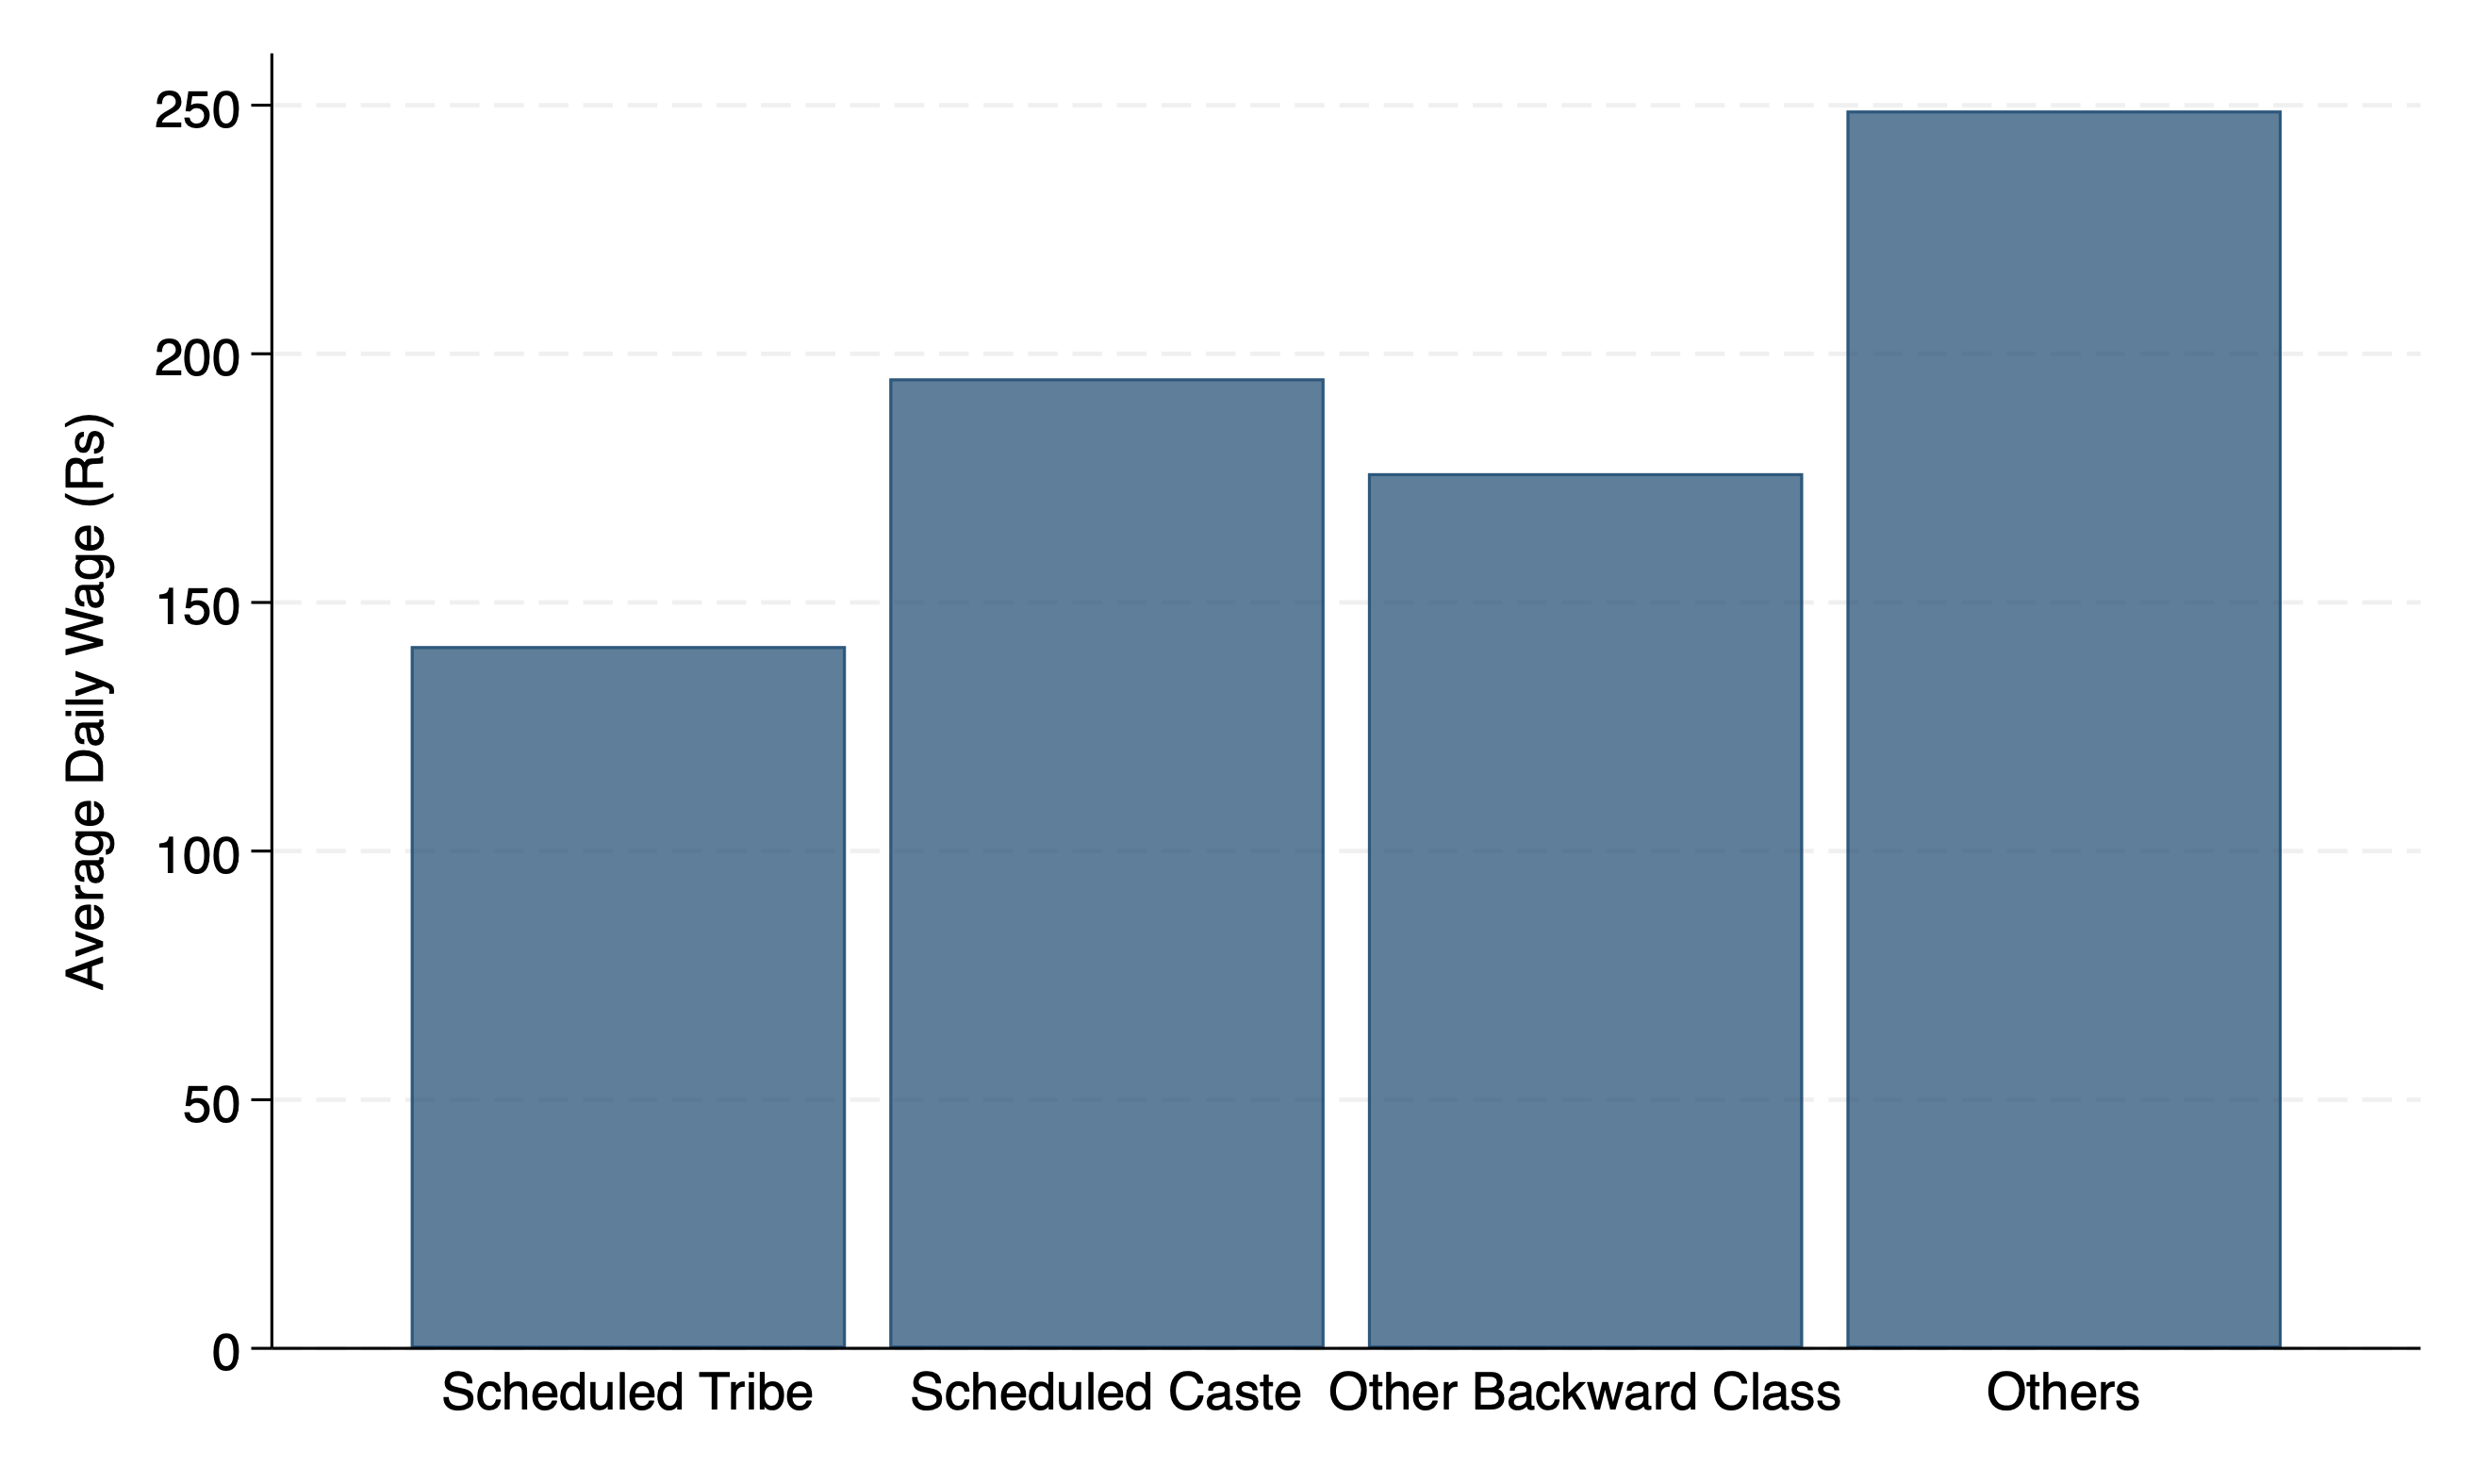
\includegraphics[scale=0.25]{daily_wage_by_caste.png}
    \caption{Average Daily Wage by Social Group}
    \label{fig:stata_graph}
\end{figure}

\subsection{Gender wage gap}
The gender wage gap is estimated using the specification:
\begin{equation} \log(wage_i) = \beta Female_i + f(age_i) + X_i + \delta_d + \delta_o + \delta_t + \epsilon_i \end{equation}
where district, occupation, and time fixed effects are included and a control for education level. Table 6 shows that the coefficient on Female is negative and statistically significant. Women earn approximately 47.2\% lower wages than men, even after controlling for observable characteristics and fixed effects. This suggests a substantial unexplained gender wage gap.


\begin{table}[htbp]\centering
\def\sym#1{\ifmmode^{#1}\else\(^{#1}\)\fi}
\caption{Linear Regression for gender wage gap}
\begin{tabular*}{0.6\hsize}{@{\hskip\tabcolsep\extracolsep\fill}l*{1}{c}}
\toprule
                &\multicolumn{1}{c}{(1)}\\
                &\multicolumn{1}{c}{Log Wage}\\
\midrule
Female (1 = yes)&   -0.472\sym{***}\\
                &  (0.016)         \\
\addlinespace
Age             &    0.014\sym{***}\\
                &  (0.000)         \\
\bottomrule
\multicolumn{2}{l}{\footnotesize FE: District, Occupation, Quarter. Clustered SE at district.}\\
\multicolumn{2}{l}{\footnotesize Education dummies included.}\\
\multicolumn{2}{l}{\footnotesize \sym{*} \(p<0.10\), \sym{**} \(p<0.05\), \sym{***} \(p<0.01\)}\\
\end{tabular*}
\end{table}
 \label{tab:wage_gap}
\subsection{Difference-in-Differences analysis} 

To understand how the January 2018 policy change in wage transparency affected the wage gap between males and females, the following DiD specification is used:
\begin{equation} \log(wage_{it}) = \beta_1 Female_i + \beta_2 Post_t + \beta_3 (Female_i \times Post_t) + X_{it} + \epsilon_{it} \end{equation}
where $Post_t$ equals 1 after January 2018. Controls include age and education level. 
The interaction term captures the change in the gender wage gap following the policy. Table 7 shows that the interaction coefficient is negative and statistically significant. Interpreted in percentage terms, this corresponds to approximately a 6.2\% additional decline in female wages relative to males in the post-policy period ($\exp(\beta_3) - 1 = -0.062$, $p = 0.011$).


The coefficient on the post-policy indicator is positive and statistically significant, suggesting that wages increased overall after 2018. However, the negative interaction term implies that these gains were not equally shared, with women benefiting less than men.

\begin{table}[htbp]\centering
\def\sym#1{\ifmmode^{#1}\else\(^{#1}\)\fi}
\caption{DiD estimates for Wage Transparency Policy}
\begin{tabular}{l*{1}{c}}
\toprule
                    &\multicolumn{1}{c}{(1)}\\
                    &\multicolumn{1}{c}{Log Wage}\\
\midrule
Female              &      -0.458\sym{***}\\
                    &     (0.029)         \\
\addlinespace
Post-policy (Jan 2018 onwards)&       0.066\sym{***}\\
                    &     (0.012)         \\
\addlinespace
Female x Post (DiD) &      -0.064\sym{**} \\
                    &     (0.026)         \\
\bottomrule
\multicolumn{2}{l}{\footnotesize Standard errors in parentheses}\\
\multicolumn{2}{l}{\footnotesize \parbox{0.9\linewidth}{District fixed effects; SE clustered at district level.}}\\
\multicolumn{2}{l}{\footnotesize \sym{*} \(p<0.10\), \sym{**} \(p<0.05\), \sym{***} \(p<0.01\)}\\
\end{tabular}
\end{table}
 

The key identifying assumption here is that of parallel trends. In the absence of the policy, male and female wages would have followed similar trajectories over time. Figure 3 suggests some divergence in male and female log wages even in the pre-policy period.

\begin{figure}[H]
    \centering
    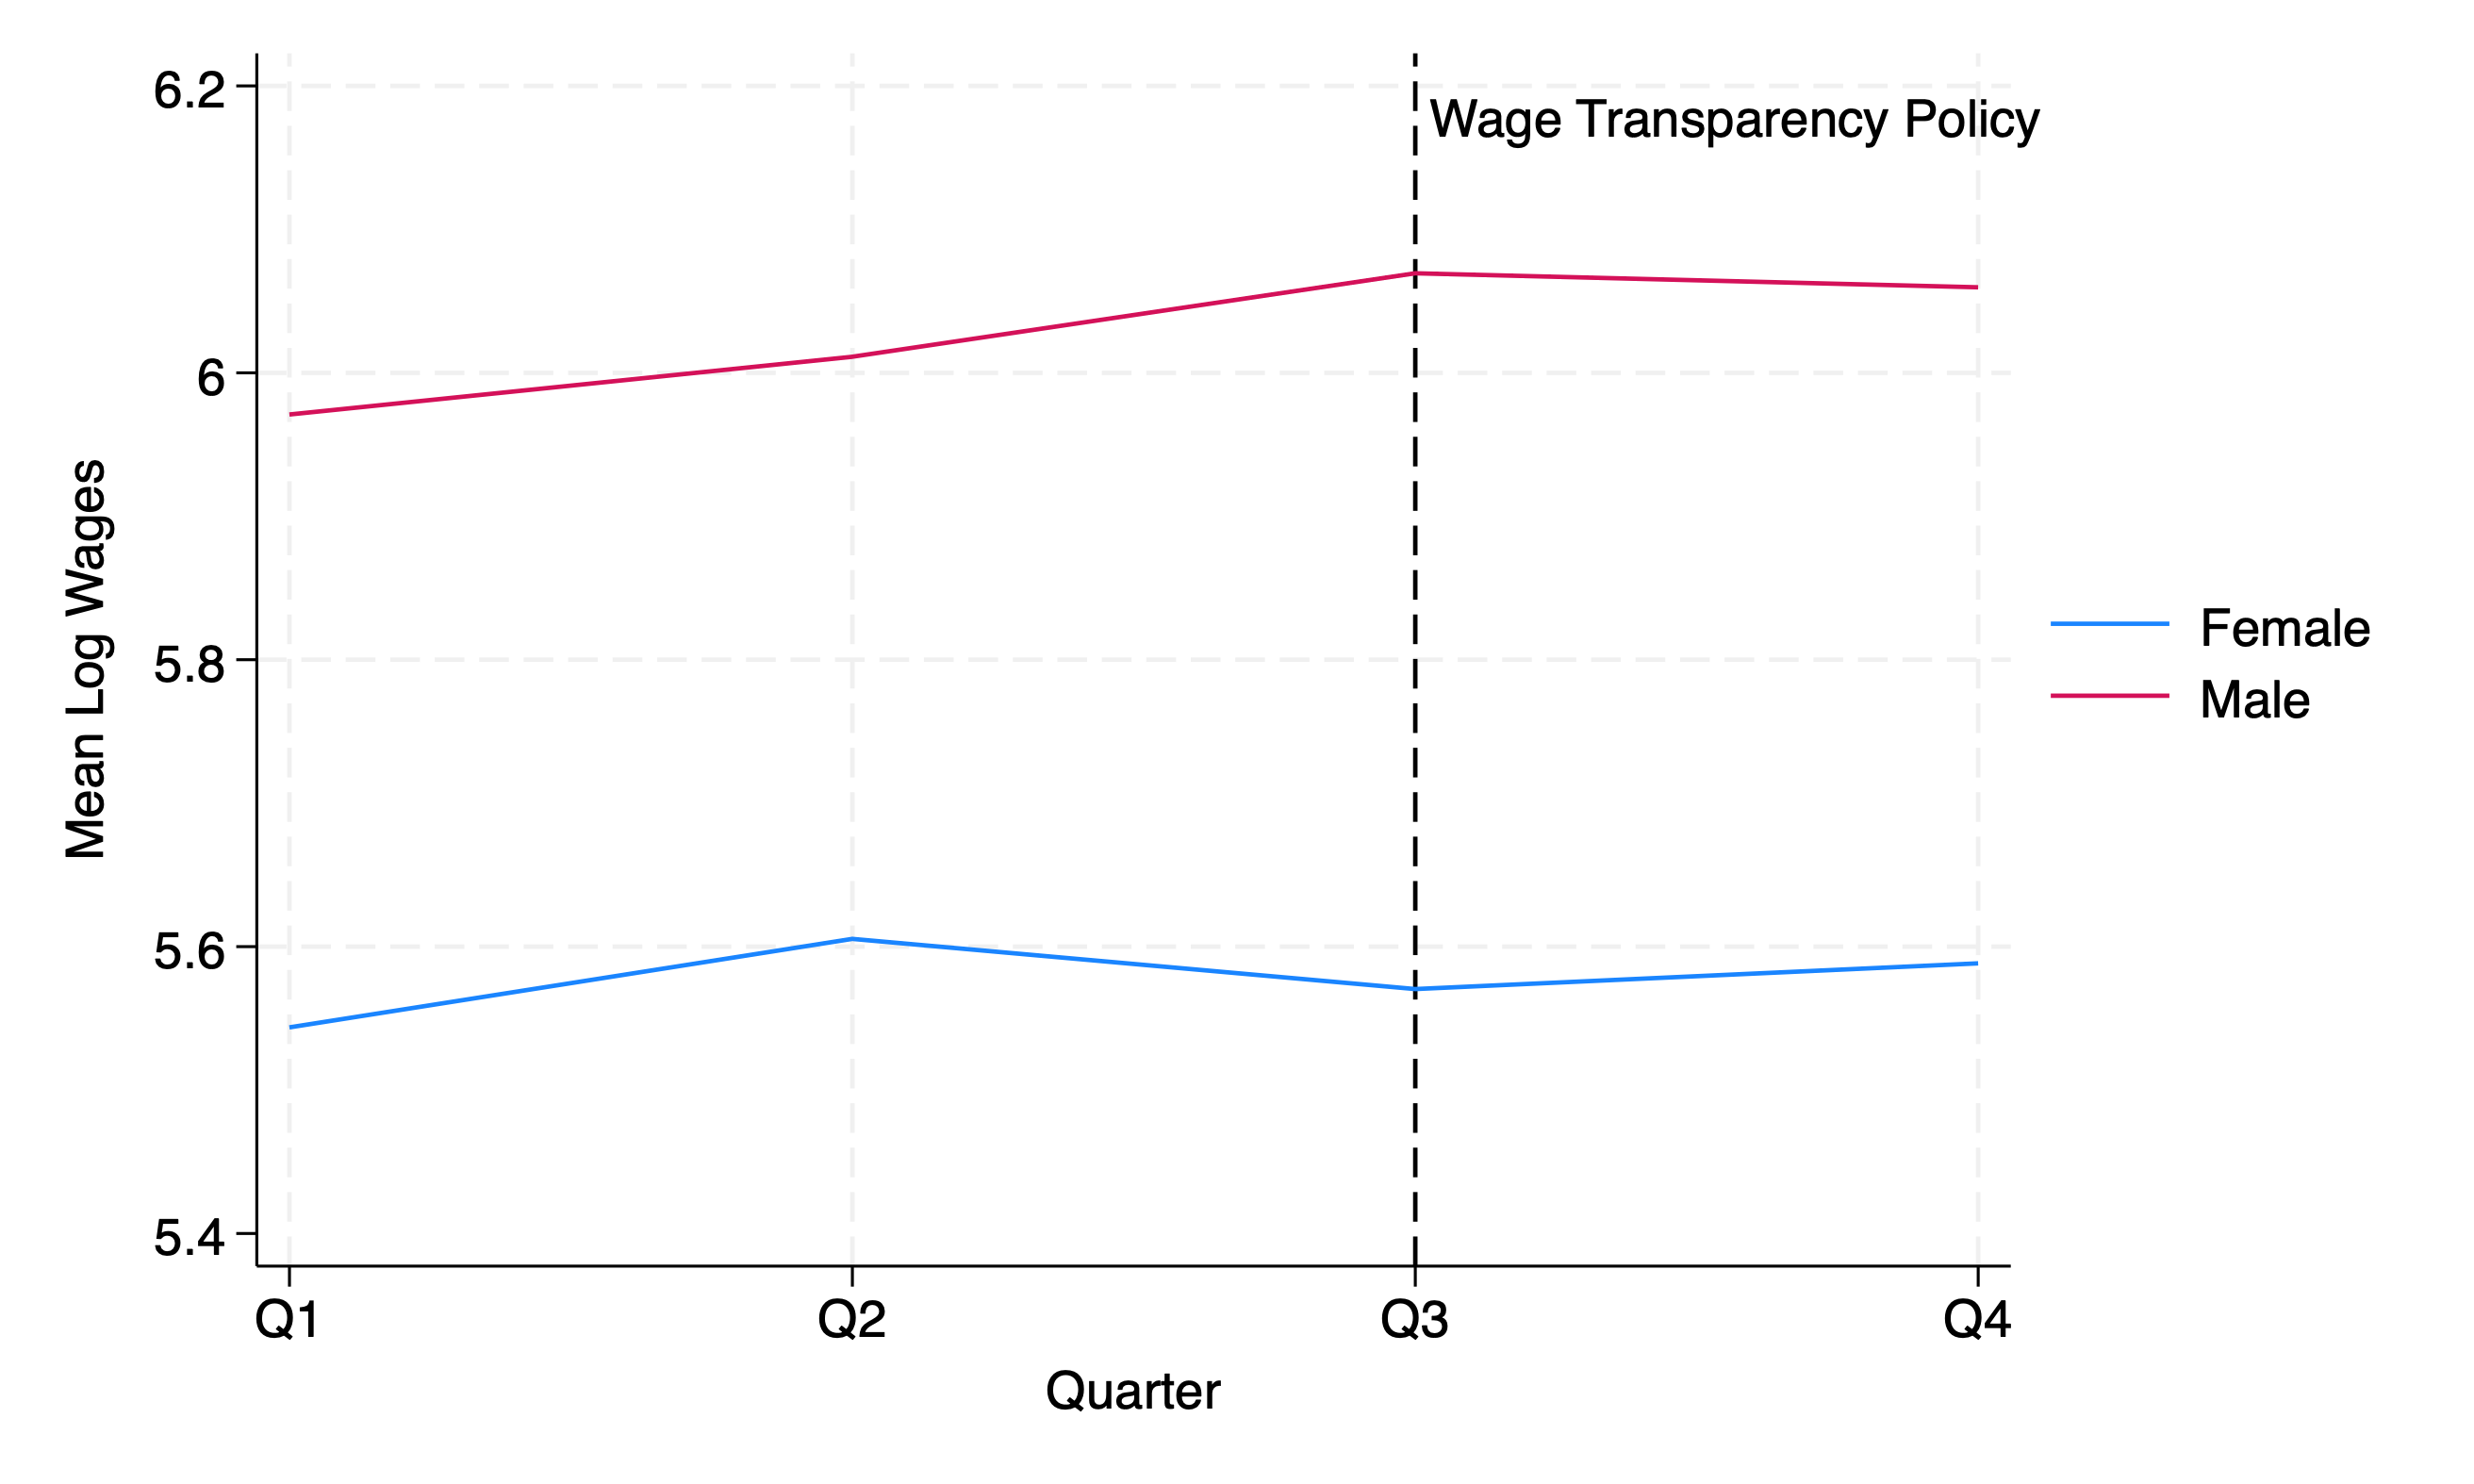
\includegraphics[scale=0.25]{did_trends.png}
    \caption{Diff-in-Diff estimation}
    \label{fig:stata_graph}
\end{figure}


\end{document}